\subsection{Structural information}
\label{ssec:action_methods_structuralinformation}

Semantic Event Chains offer a good understanding of top or bottom and the now introduced Enriched Semantic Event Chains additionally express ``left'' and ``right''.
This gives valuable information on how to execute an action, but very little information, whether an action is feasible.
In this chapter structural topologies of object graphs are analyzed.
For visualization, we will assume in this chapter that object segmentation and recognition performs in a perfect manner.
Furthermore, one must assume that the support of an object is always below the object itself and that the object recognition software provides knowledge about the supporting objects, \eg if a table is present, the table is marked as supporting object.
This also marks the constraints of this approach: Hanging structures are not analyzed here.

As noted in \secref{ssec:action_methods_actioncategories}, an action will always be performed on the \emph{main} object.
To analyze the structure around the \emph{main} object, subgraphs are created, where one subgraph always holds the support and the \emph{main} object, and up to one other object, which is called \emph{primary} object.
Remarkably, there are only three possible topological subgraphs to which all scenes that include the \emph{main} object can be reduced.
These three possible cases are shown in \figref{fig:sec_structuralinformation_structures}:

\begin{enumerate}
  \item The \emph{main} object has only one touching relation. The touched object is a support (see \figref{fig:sec_structuralinformation_structures_1}). A real world example could be a plate lying on a table.
  \item The \emph{main} object has two touching relations. One is a support, the second one is another object, which is also touching a support (see \figref{fig:sec_structuralinformation_structures_2}). A real world scene could be a plate and a cup on a table, both are touching each other.
  \item The \emph{main} object has two touching relations. One is a support, the second one is another object, which does not touch a support (see \figref{fig:sec_structuralinformation_structures_3}). Lastly, this structure could emerge from a plate with an apple on top; the plate being the \emph{main} object here.
\end{enumerate}

\begin{figure}[]
  \begin{subfigure}[]{0.3\textwidth}
    \centering
    % Define block styles
\tikzstyle{block} = [rectangle, fill=white, text centered, minimum height=0.5em, rounded corners=false]
\tikzstyle{arrow} = [draw, -latex]

\definecolor{red1}{RGB}{160,0,0}
\definecolor{green1}{RGB}{0,160,0}
\definecolor{blue1}{RGB}{0,0,160}

	      
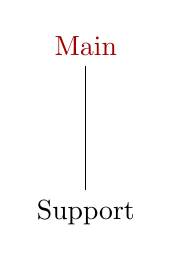
\begin{tikzpicture}[node distance=6em, auto]
	% single
	\node [block] (S1) {Support};
	\node [block, above of=S1] (M1) {\textcolor{red1}{Main}};

	\draw [] (S1.north) to (M1.south);
\end{tikzpicture}

    \caption{Example: Plate on a table.}
    \label{fig:sec_structuralinformation_structures_1}
  \end{subfigure}
  \hfill
  \begin{subfigure}[]{0.3\textwidth}
    \centering
    % Define block styles
\tikzstyle{block} = [rectangle, fill=white, text centered, minimum height=0.5em, rounded corners=false]
\tikzstyle{arrow} = [draw, -latex]

\definecolor{red1}{RGB}{160,0,0}
\definecolor{green1}{RGB}{0,160,0}
\definecolor{blue1}{RGB}{0,0,160}

	      
\begin{tikzpicture}[node distance=6em, auto]
	% touching
	\node [block, right of=S1, node distance=5cm] (S2) {Support};
	\node [block, above of=S2, xshift=-1cm] (M2) {\textcolor{red1}{Main}};
	\node [block, above of=S2, xshift= 1cm] (Se2) {Primary};

	\draw [] (S2.north) to (M2.south);
	\draw [] (S2.north) to (Se2.south);
	\draw [] (M2.east) to (Se2.west);
\end{tikzpicture}

    \caption{Example: Plate next to a cup on a table.}
    \label{fig:sec_structuralinformation_structures_2}
  \end{subfigure}
  \hfill
  \begin{subfigure}[]{0.3\textwidth}
    \centering
    % Define block styles
\tikzstyle{block} = [rectangle, fill=white, text centered, minimum height=0.5em, rounded corners=false]
\tikzstyle{arrow} = [draw, -latex]

\definecolor{red1}{RGB}{160,0,0}
\definecolor{green1}{RGB}{0,160,0}
\definecolor{blue1}{RGB}{0,0,160}

	      
\begin{tikzpicture}[node distance=6em, auto]
	% tower
	\node [block, right of=S2, node distance=5cm] (S3) {Support};
	\node [block, above of=S3, node distance=3em] (M3) {\textcolor{red1}{Main}};
	\node [block, above of=M3, node distance=3em] (Se3) {Primary};

	\draw [] (S3.north) to (M3.south);
	\draw [] (M3.north) to (Se3.south);
\end{tikzpicture}

    \caption{Example: Apple on a plate on a table.}
    \label{fig:sec_structuralinformation_structures_3}
  \end{subfigure}
  \caption{Only these three subgraphs may exist around the \emph{main} object. Any graph structure, which contains at least a \emph{main} object and its support, can be reduced to a series of these subgraphs. Any subgraph consists of the \emph{main} object, its support, and up to one more object.}
  \label{fig:sec_structuralinformation_structures}
\end{figure}

Next, a real-world example as shown in \figref{fig:sec_structuralinformation_example_scene} is analyzed.
The computer vision system delivers a low level graph structure, but also two pieces of high level information: which object is the table/the support and what is the \emph{main} object.
The supporting object is important, because it is always below all other objects.
The objects are named analogously to \secref{ssec:action_methods_actioncategories}, meaning the manipulated object is called \emph{main} object.
The resulting graph is decomposed into two subgraphs: one tower-like structure and one structure where the \emph{primary} is situated next to the \emph{main} object.
\glspl{ac:sec} do not offer information about size, and the bottle O$_1$ could be far away of the plate -- it is therefore disregarded.

\begin{figure}
  \centering
  \begin{subfigure}[]{0.475\textwidth}
    \centering
    \includegraphics[width=\textwidth]{./figures/sec/structuralinformation_example_scene.jpg}
    \caption{The original scene as viewed by the robot. A higher level algorithm (or human) chooses the plate as \emph{main} object to manipulate}
    \label{fig:sec_structuralinformation_example_scene}
  \end{subfigure}\hfill%
  \begin{subfigure}[]{0.475\textwidth}
    \centering
    % Define block styles
\tikzstyle{block} = [rectangle, fill=white, text centered, minimum height=0.5em, rounded corners=false]
\tikzstyle{arrow} = [draw, -latex]
\tikzstyle{background} = [draw, rectangle, text centered, text width=3.5cm, minimum height=4.7cm, color=white]

\usetikzlibrary{decorations.pathreplacing}

\definecolor{red1}{RGB}{160,0,0}
\definecolor{green1}{RGB}{0,160,0}
\definecolor{blue1}{RGB}{0,0,160}

	      
\begin{tikzpicture}[node distance=3em, auto]
	% Example
	\node [block] (S01) {Table};
	\node [block, above of=S01] (M01) {\textcolor{red1}{Plate}};
	\node [block, left of=M01, node distance=5em]  (O01) {Bottle};
	\node [block, right of=M01, node distance=5em] (O02) {Knife};
	\node [block, above of=M01] (O03) {Apple};

	\draw [] (S01.north) to (M01.south);
	\draw [] (S01.north west) to (O01.south east);
	\draw [] (S01.north east) to (O02.south west);
	\draw [] (M01.north) to (O03.south);
	\draw [] (M01.east) to (O02.west);

  \node[background] at (M01) {};
\end{tikzpicture}

    \caption{The extracted graph relations after object classification. Plate is recognized as \emph{main} object.}
  \end{subfigure}\vspace{0.5cm}\\%
  \begin{subfigure}[]{\textwidth}
    \centering
    % Define block styles
\tikzstyle{block} = [rectangle, fill=white, text centered, minimum height=0.5em, rounded corners=false]
\tikzstyle{arrow} = [draw, -latex]

\usetikzlibrary{decorations.pathreplacing}

\definecolor{red1}{RGB}{160,0,0}
\definecolor{green1}{RGB}{0,160,0}
\definecolor{blue1}{RGB}{0,0,160}

	      
\begin{tikzpicture}[node distance=3em, auto]
	% full
	\node [block, below of=S01, node distance=10em] (S1) {Support};
	\node [block, above of=S1] (M1) {\textcolor{red1}{Main}};
	\node [block, left of=M1, node distance=4em]  (O11) {O$_1$};
	\node [block, right of=M1, node distance=4em] (O12) {O$_2$};
	\node [block, above of=M1] (O13) {O$_3$};

	\draw [] (S1.north) to (M1.south);
	\draw [] (S1.north west) to (O11.south east);
	\draw [] (S1.north east) to (O12.south west);
	\draw [] (M1.north) to (O13.south);
	\draw [] (M1.east) to (O12.west);

	% arrow
	\draw [arrow] (O12.east)++(1.5em,0em) to ++(3.5em,0em);

	% {
	\draw [decorate, decoration={brace, amplitude=10pt}, right of=O12, xshift=2.5em, node distance=3em] (7em,-11.0em) -- (7em,-3.0em) node (klammer1) [black,midway] {};

	% 3
	%\node [block, right of=S1, node distance=10em] (S3) {S};
	%\node [block, above of=S3] (M3) {\textcolor{red1}{M}};
	%\node [block, left of=M3]  (O31) {O};

	%\draw [] (S3.north) to (M3.south);
	%\draw [] (S3.north west) to (O31.south east);

	% +
	%\node [block, right of=M3, node distance=1.5em] (+) {+};

	% 1
	\node [block, right of=S1, node distance=15em] (S2) {Support};
	\node [block, above of=S2] (M2) {\textcolor{red1}{Main}};
	\node [block, above of=M2] (O23) {Primary};

	\draw [] (S2.north) to (M2.south);
	\draw [] (M2.north) to (O23.south);

	% +
	\node [block, right of=M2, node distance=3em, yshift=-0.35em] (+) {,};

	% 2
	\node [block, right of=S2, node distance=6em] (S3) {Support};
	\node [block, above of=S3] (M3) {\textcolor{red1}{Main}};
	\node [block, right of=M3, xshift=2em] (O32) {Primary};

	\draw [] (S3.north) to (M3.south);
	\draw [] (S3.north east) to (O32.south west);
	\draw [] (M3.east) to (O32.west);

	% {
	\draw [decorate, decoration={brace, amplitude=10pt, mirror}, right of=O32] (25.7em,-11.0em) -- (25.7em,-3.0em) node [black,midway] {};
\end{tikzpicture}

    \caption{The abstract graph is cut into two subgraphs around the \emph{main} object, the plate. As the bottle has no direct connection to the plate, no subgraph is generated. As the subgraph consists of at least the support and \emph{main} object, the third object is automatically named \emph{primary} object, see \secref{ssec:action_methods_affordanceofsemanticeventchains}. ``O'' stands for other, not closer defined objects.}
  \end{subfigure}
  \caption{A scene, as recorded by a robot is analyzed and a graph structure is generated. As \emph{main} object the plate is chosen by either human or higher level algorithms. For each object around the \emph{main} object a subgraph is generated.}
  \label{fig:sec_structuralinformation_example}
\end{figure}

Now, the complex graph structure is broken down to much simpler subgraphs.
It is already well known that the mere existence of objects already suggests scenes~\cite{zhu2014reasoning}: For example, an image of a plate, cutlery, a roll, and a glass of juice will more likely show a breakfast scene, than an image of a supermarket.
But an isle inside a supermarket could show the same objects from the breakfast scene (and probably many more at the same time) in a different context.
One can easily see, that a scene's affordance heavily depends on discriminative spatial layouts~\cite{tran2017recognition, lin2014learning}.
In the next section, it is analyzed how the subgraphs can be used as additional features to \glspl{ac:esec} to compute a scene's affordance.
